\documentclass{beamer}
% pdfpc --notes=right slides.pdf
% "tecla p": para pausar el cronometro
\mode<presentation> {
	\usetheme{CambridgeUS}
	\usecolortheme{crane} % color naranja
}

\setbeamercolor{titlelike}{parent=structure,bg=yellow!85!orange} % Cambia el color de la caja del título de la página inicial

\setbeamertemplate{navigation symbols}{} % ocultar iconos de navegación
\setbeamerfont{subsection in toc}{size=\small} % reducir tamaño en TOC
\setbeamerfont{date}{size=\tiny}
\usepackage[spanish]{babel}
\usepackage[utf8]{inputenc}
\usepackage{graphicx}
\usepackage{booktabs}
\usepackage{hyperref}
\usepackage{multicol}
\usepackage{pgfpages}
\usepackage{listings}
\usepackage{multimedia}
\usepackage[export]{adjustbox}
\usepackage{outlines} % Para poner bullets tabulados (\1 \2 \3 ...) y no items

\usepackage{array,tabularx} % para tabular leyenda de ecuaciones
\newenvironment{conditions*} % entorno de "leyenda de ecuación"
	{\par\vspace{\abovedisplayskip}\noindent
	 \tabularx{\columnwidth}{>{$}l<{$} @{\ : } >{\raggedright\arraybackslash}X}}
	{\endtabularx\par\vspace{\belowdisplayskip}}
	
% USO DE NOTAS
\setbeameroption{hide notes} % Para mostrar u ocultar (hide/show)
% \setbeameroption{show only notes} % Mostrar solo las notas
% \setbeameroption{show notes on second screen=right} % Mostrar notas en otra pantalla
\setbeamertemplate{note page}{ % asi solo muestro el texto de las notas
	\insertnote%
}

\hypersetup{
	pdftitle={Defensa de trabajo de fin de grado de Álvaro Mariscal Ávila},
	pdfauthor={Álvaro Mariscal Ávila},
	pdfsubject={Conducción autónoma sobre plataforma real y simulada con seguimiento de carril e identificación de señales de tráfico y peatones mediante redes neuronales},
	pdfkeywords={robotics, vision, sensors, actuators, neural networks},
	pdfproducer={pdfLaTeX},
	colorlinks=true,
	linkcolor=blue
}
% =========

\title[Conducción autónoma con redes neuronales]{Conducción autónoma sobre plataforma real y simulada con seguimiento de carril e identificación de señales de tráfico y peatones mediante redes neuronales} % El título reducido aparece en la parte inferior de todas las diapositivas
% El título completo aparece solo en la diapositiva de portada
\author[Álvaro Mariscal Ávila]{Álvaro Mariscal Ávila}
\institute[URJC]
{
\textit{\href{mailto:a.mariscal.2018@alumnos.urjc.es}{\color{blue}{\underline{a.mariscal.2018@alumnos.urjc.es}}}}\\
\vspace{0.5cm}

\includegraphics[width=3cm]{figs/logo-urjc}\\
\vspace{1cm}
Trabajo fin de grado
}
\date{xx de xxxxxxx de 2022}
% =========

% ========= COMIENZO DEL DOCUMENTO
\begin{document}

% ========= Portada inicial con notas
\begin{frame}[plain] % plain: quita header y footer
	\large{\titlepage}
	\note[item]{En esta presentación voy a hablar sobre...}
	\note[item]{En primer lugar...}
\end{frame}

% ========= Licencia
\begin{frame}
% Este diseño se corresponde con la licencia CC-BY-NC-SA.
% Por supuesto, puedes poner la licencia que mejor se adapte al propósito de tu trabajo.
% Recuerda que, si no se especifica ninguna licencia, esta -como cualquier creación artística- pasaría a estar licenciada con todos los derechos reservados (copyright).

\vspace{5cm}

\begin{flushright}

\begin{figure}

\includegraphics[width=0.10\textwidth,right]{figs/by-nc-sa.png}
\end{figure}

\vspace{0.2cm}

{\tiny 
(CC) \textbf{Julio Vega}\\ % TODO: pon aquí tu nombre cuando hagas el documento
\vspace{0.5cm}
\emph{
Este trabajo se entrega bajo licencia \href{https://creativecommons.org/licenses/by-nc-sa/3.0/es/}{CC BY-NC-SA}. \\
Usted es libre de \textit{(a) compartir}: copiar y redistribuir el material en \\
cualquier medio o formato; y \textit{(b) adaptar}: remezclar, transformar \\
y crear a partir del material. El licenciador no puede revocar estas \\
libertades mientras cumpla con los términos de la licencia. \\}
}

\end{flushright}


\end{frame}

% ========= Índice o tabla de contenidos (TOC)
\begin{frame}
\frametitle{Contenidos}
% \begin{multicols}{2} % si tengo muchas secciones, lo parte en dos columnas
	\tableofcontents[hideallsubsections] % no muestra subsecciones
% \end{multicols}
\note[item]{La presentaci\'on esta dividida en cuatro partes.}
\end{frame}

% ========= Diapositiva "vacía" de comienzo de sección:
\section*{}
\begin{frame}{}
	\centering \Huge
	\emph{Introducción}
\note[item]{Comencemos con la introducción.}
\end{frame}

%%%%%%%%%%%%%%%%%%%%%%%%%%%%%%%%%%%%%%%%%%%%%%%%%%%%%%%%%%%%%%%%%% Capítulo 1 %%%%%%%%%%%%%%%%%%%%%%%%%%%%%%%%%%%%%%%%%%%%%%%%%%%%%%%%%%%%%%%%%%%%% 

\section{Introducción}
\subsection{Contexto general}
\begin{frame}
	\frametitle{Inteligencia artificial}
	\begin{figure}
	\centering
	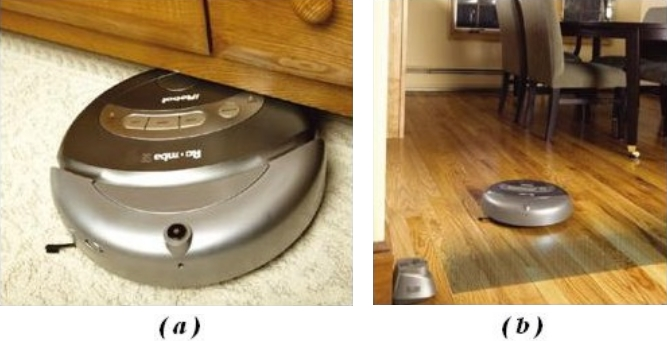
\includegraphics[width=8cm]{figs/roomba}
	\end{figure}
\end{frame}

\begin{frame}
	\frametitle{Visión artificial}
	\begin{itemize}
	\item La \textcolor{red}{tecnología} está cada vez más presente en la vida cotidiana.
	\item Los robots de servicio aparecen en el \textcolor{blue}{mercado}.
	\item La \textcolor{red}{domótica} presenta cada vez más aplicaciones domésticas.
	\end{itemize}
\end{frame}

\begin{frame}
	\frametitle{Deep Learning}
	\begin{figure}
	\centering
	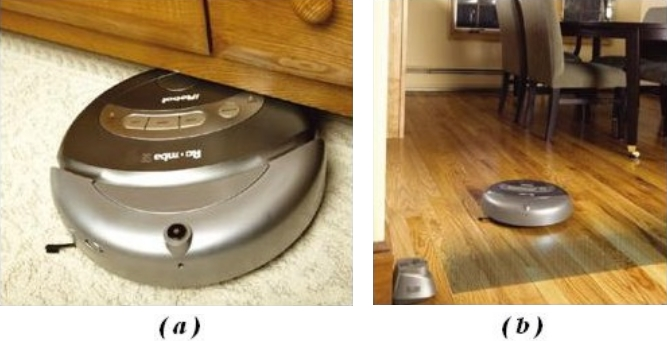
\includegraphics[width=8cm]{figs/roomba}
	\end{figure}
\end{frame}

\subsection{Contexto específico}
\begin{frame}
	\frametitle{Coches autónomos}
	\begin{block}{Primera revolución industrial de 1800}
	Productos fabricados por \textcolor{blue}{máquinas}. La \textcolor{red}{máquina de vapor} fue clave.
	\end{block}
\end{frame}

\begin{frame}
	\frametitle{AMRs}
	\begin{block}{Primera revolución industrial de 1800}
	Productos fabricados por \textcolor{blue}{máquinas}. La \textcolor{red}{máquina de vapor} fue clave.
	\end{block}
\end{frame}

%%%%%%%%%%%%%%%%%%%%%%%%%%%%%%%%%%%%%%%%%%%%%%%%%%%%%%%%%%%%%%%%%% Capítulo 2 %%%%%%%%%%%%%%%%%%%%%%%%%%%%%%%%%%%%%%%%%%%%%%%%%%%%%%%%%%%%%%%%%%%%% 

\section*{}
\begin{frame}{}
	\centering \Huge
	\emph{Objetivos}
	\note[item]{Objetivos.}
\end{frame}

\section{Objetivos}
\subsection{Descripción del problema}
\begin{frame}
	\frametitle{Descripción del problema}
	\begin{outline}
	\1 relación
	\end{outline}
\end{frame}

\subsection{Requisitos}
\begin{frame}
	\frametitle{Requisitos}
	\begin{outline}
	\1 relación
	\end{outline}
\end{frame}

%%%%%%%%%%%%%%%%%%%%%%%%%%%%%%%%%%%%%%%%%%%%%%%%%%%%%%%%%%%%%%%%%% Capítulo 3 %%%%%%%%%%%%%%%%%%%%%%%%%%%%%%%%%%%%%%%%%%%%%%%%%%%%%%%%%%%%%%%%%%%%% 

\section*{}
\begin{frame}{}
	\centering \Huge
	\emph{Plataforma de desarrollo}
	\note[item]{Pasemos ahora a comentar los objetivos que nos hemos con este trabajo.}
\end{frame}

\section{Plataforma de desarrollo}
\subsection{Hardware}
\begin{frame}
		\frametitle{Hardware}
	\begin{enumerate}
	\item Crear una herramienta multiplataforma.
	\item Sin necesidad de instalación.
	\item Toda ejecución vía web.
	\end{enumerate}
\end{frame}

\subsection{Software}
\begin{frame}
	\frametitle{Software}
	\begin{enumerate}
	\item Crear una herramienta multiplataforma.
	\item Sin necesidad de instalación.
	\item Toda ejecución vía web.
	\end{enumerate}
\end{frame}

%%%%%%%%%%%%%%%%%%%%%%%%%%%%%%%%%%%%%%%%%%%%%%%%%%%%%%%%%%%%%%%%%% Capítulo 4 %%%%%%%%%%%%%%%%%%%%%%%%%%%%%%%%%%%%%%%%%%%%%%%%%%%%%%%%%%%%%%%%%%%%% 

\section*{}
\begin{frame}{}
	\centering \Huge
	\emph{Sistema de conducción autónoma}
	\note[item]{Una vez descritos los objetivos, veamos qué hemos hecho para alcanzarlos.}
\end{frame}

\section{Sistema de conducción autónoma}
\subsection{Entorno simulado}
\begin{frame}
	\frametitle{Modelo}
	\begin{itemize}
	\item Se usa una matriz $RT (4x4)$ en lugar de $R$ y $T$.
	\item La matriz $RT$ rota $\theta$ grados en los ejes $X$, $Y$ y $Z$:
	\end{itemize}
\end{frame}

\begin{frame}
	\frametitle{Resistencia de un material}
	\begin{outline}
	\1 Si material piezoresistivo se deforma, cambia su resistencia eléctrica.
	donde:
	\begin{conditions*}
	R & resistencia del material $[\Omega]$\\
	\rho & resistividad $[\Omega-m]$\\
	l & longitud $[m]$\\
	A & área de sección transversal $[m^2]$
	\end{conditions*}
	\1 El cambio de resistencia se obtiene a partir de:
	\end{outline}
\end{frame}

\subsection{Entorno real}
\begin{frame}
	\frametitle{Circuito}
	\begin{itemize}
	\item Se usa una matriz $RT (4x4)$ en lugar de $R$ y $T$.
	\item La matriz $RT$ rota $\theta$ grados en los ejes $X$, $Y$ y $Z$:
	\end{itemize}
\end{frame}

\begin{frame}
	\frametitle{Redes neuronales en el entorno real}
	\begin{outline}
	\1 Si material piezoresistivo se deforma, cambia su resistencia eléctrica.
	donde:
	\begin{conditions*}
	R & resistencia del material $[\Omega]$\\
	\rho & resistividad $[\Omega-m]$\\
	l & longitud $[m]$\\
	A & área de sección transversal $[m^2]$
	\end{conditions*}
	\1 El cambio de resistencia se obtiene a partir de:
	\end{outline}
\end{frame}

%%%%%%%%%%%%%%%%%%%%%%%%%%%%%%%%%%%%%%%%%%%%%%%%%%%%%%%%%%%%%%%%%% Capítulo 5 %%%%%%%%%%%%%%%%%%%%%%%%%%%%%%%%%%%%%%%%%%%%%%%%%%%%%%%%%%%%%%%%%%%%% 

\section*{}
\begin{frame}{}
	\centering \Huge
	\emph{Conclusiones}
	\note[item]{Para acabar esta presentación, vamos a repasar lo hecho, unas breves conclusiones y las líneas futuras.}
\end{frame}

\section{Conclusiones}
	\begin{frame}
	\frametitle{Conclusiones}
	\begin{itemize}
	\item Se usa una matriz $RT (4x4)$ en lugar de $R$ y $T$.
	\item La matriz $RT$ rota $\theta$ grados en los ejes $X$, $Y$ y $Z$:
	\end{itemize}
\end{frame}

\subsection{Líneas futuras}
\begin{frame}
	\frametitle{Líneas futuras}
	\begin{itemize}
	\item Se usa una matriz $RT (4x4)$ en lugar de $R$ y $T$.
	\item La matriz $RT$ rota $\theta$ grados en los ejes $X$, $Y$ y $Z$:
	\end{itemize}
\end{frame}

\begin{frame}[plain]
	\large{\titlepage}
	\note[item]{Y hasta aquí mi exposición.}
	\note[item]{Quedo a disposición del tribunal...}
\end{frame}

\end{document}
